\documentclass[a4paper,12pt, twoside]{article}
%\documentclass[a4paper,12pt, twoside]{book}

\usepackage[papersize={210mm,297mm},tmargin=20mm,bmargin=20mm,lmargin=20mm,rmargin=20mm]{geometry}

\usepackage[utf8]{inputenc}
%https://mirror.hmc.edu/ctan/macros/latex/contrib/babel-contrib/turkish/turkish.pdf
\usepackage[english]{babel}
%\usepackage[T1]{fontenc}

\usepackage{enumitem}

\usepackage{amsmath,amssymb,mathabx}%\for eqref
\usepackage{lscape}
\usepackage{tcolorbox}

\usepackage{hyperref}
\hypersetup{
    colorlinks,
    citecolor=black,
    filecolor=black,
    linkcolor=blue,
    urlcolor=red}
  

%\usepackage{svg}
%%% https://tex.stackexchange.com/questions/122871/include-svg-images-with-the-svg-package/129854
\usepackage{graphicx}
\graphicspath{ {./figurler/} }

\usepackage[colorinlistoftodos]{todonotes}
\usepackage{fancyhdr}

\usepackage{indentfirst}
%% paragraf girintisi
\setlength{\parindent}{5ex}

%% Daha sonra yazılacak kısımları not düşmek için...
\newcommand{\YAZILACAK}{{\vspace{18pt}\bf\Large \color{red} YAZILACAK}}


\pagestyle{fancy}
\fancyhf{}
\lhead{ Kuantum Fiziği }
\chead{\thepage}
\rhead{Mesut Karakoç}
\lfoot{Akdeniz Üniversitesi}
\cfoot{}
%\rfoot{BF}

\title{Akdeniz Üniversitesi\\ Fen Fakültesi - Fizik Bölümü\\FİZ319 Kuantum Fiziği Ders Notları}

\author{\setlength{\unitlength}{6mm}
\begin{picture}(10,10)
\put(1.1,0){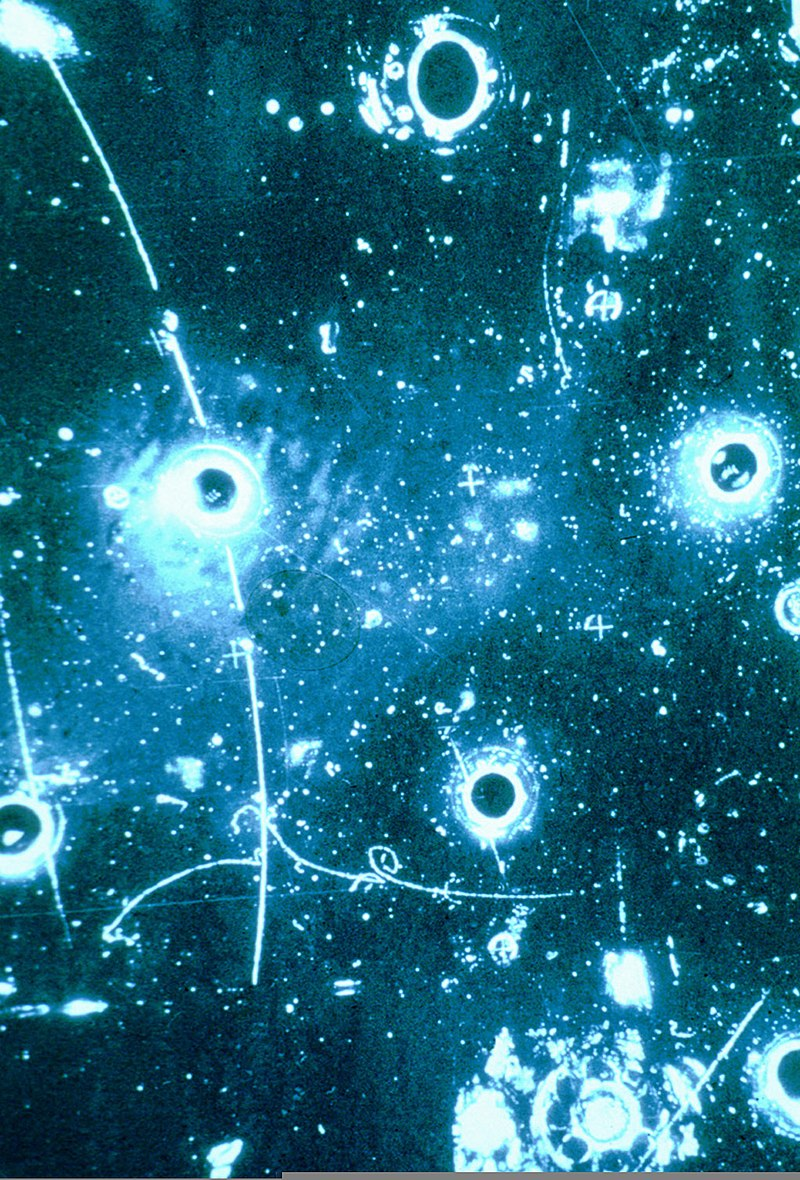
\includegraphics[width=4.5cm]{Leptonic_event_in_Gargamelle_bubble_chamber.jpg}}
\end{picture} \\ Doç. Dr. Mesut Karakoç}


\date{\today}

\begin{document}

%% Turkish babel problem
%% https://tex.stackexchange.com/questions/160385/newgeometry-doesnt-work-with-turkish-babel-package
%%\shorthandoff{=}% Make = not active any more

\maketitle

\newpage

% change name to "İçindekiler"
\renewcommand{\contentsname}{İçindekiler}
\tableofcontents{}

\listoffigures
 
\listoftables

\newpage

{
\hspace{.5\textwidth}
\begin{minipage}{.5\textwidth}
\raggedleft
If all this damned quantum jumps were really to stay, I should be
sorry I ever got involved with quantum theory.

—Erwin Schrödinger
\cite{book:Ficek}

%% Latince için
%% post iacturam quis non sapit!
%% Who is not wise after he has lost something?
%% https://quizlet.com/23756827/latin-proverbs-h-flash-cards/
\end{minipage}
}

\setcounter{section}{2} %% THIS WILL BE DELETED when all chapters merged!
\section{Schrödinger Denkleminin Ayrıştırılması, Özdeğerleri ve Özfonksiyonları}

Bu bölümde bir parçacığın veya sistemin etkisinde olduğu potansiyelin $V(x)$ zamandan bağımsız olması halinde, Schrödinger denkleminin sadece konum ve sadece zaman değişkenlerini içeren iki çiftlenmiş denklem seti halinde yazılabileceğini göreceğiz. Sadece konum değişkenine bağlı olarak yazılan yeni denklemi zamandan bağımsız Schrödinger denklemi olarak adlandırıyoruz. Devamında zamandan bağımsız denklem için özdeğer, özfonksiyon kavramlarını tartışacağız ve bazı potansiyeller için bu denklemin çözümlerini inceleyeceğiz. 

\subsection{Zamandan Bağımsız Schrödinger Denklemi}
%%
Bir önceki bölümde elde ettiğimiz zamana bağlı Schrödinger denklemini \emph{Hamilton} işlemcisini kullanarak,
%%
\begin{equation}
\hat H \psi ( x , t ) = i \hbar \frac { \partial \psi ( x , t ) } { \partial t }
\label{eq:time_depended_schrodinger_eq_op_form}
\end{equation}
%%
şeklinde yazabileceğimizi ve dalga fonksiyonlarıyla açık halini de, 
%%
\begin{equation}
- \frac { \hbar ^ { 2 } } { 2 m } \frac { \partial ^ { 2 } \psi ( x , t ) } { \partial x ^ { 2 } } + V ( x ) \psi ( x , t ) = i \hbar \frac { \partial \psi ( x , t ) } { \partial t }
\label{eq:time_depended_schrodinger_eq}
\end{equation}
%%
şeklinde yazabileceğimizi görmüştük.  Yukarıda tekrar yazdığımız zamana bağlı Schrödinger denklemi  bir kısmi diferansiyel denklemdir.  Kısmi diferansiyel denklemlerin birden çok bağımsız değişkenleri olur.   Bu nedenle genellikle  kısmi diferansiyel denklemleri çözmek kolay olmayabilir.  Fakat bizim inceleyeceğimiz durumda V(x)  potansiyeli zamandan bağımsız olduğundan denklemi sadece zamanı ve sadece konuma bağlı iki adi diferansiyel denkleme    dönüştürebiliriz. 
%%
\begin{equation}
\psi ( x , t ) = T ( t ) u ( x )
\label{eq:separation_of_wave_func}
\end{equation}

Bu dönüşümü gerçekleştirebilmek için $\psi ( x , t )$'nin yukarıdaki gibi iki fonksiyonun çarpımı şeklinde yazılabileceğini kabul edeceğiz. Dalga fonksiyonunun bu halin zamana bağlı Schrödinger denkleminde kullanırsak,
%%
\begin{equation*}
i \hbar u ( x ) \frac { d T ( t ) } { d t } = \left\{ - \frac { \hbar ^ { 2 } } { 2 m } \frac { d ^ { 2 } u ( x ) } { d x ^ { 2 } } + V ( x ) u ( x ) \right\} T ( t )
\end{equation*}
%%
denklemine ulaşırız. Bu denklemin her iki tarafını $T ( t ) u ( x )$ ifadesine bölersek,
%%
\begin{equation}
i \hbar \frac { 1 } { T ( t ) } \frac { d T ( t ) } { d t } = \frac { 1 } { u ( x ) } \left\{ - \frac { \hbar ^ { 2 } } { 2 m } \frac { d ^ { 2 } u ( x ) } { d x ^ { 2 } } + V ( x ) u ( x ) \right\}
\label{eq:sch_separeted}
\end{equation}
%%
her iki tarafı sadece bir bağımsız değişkene bağlı bir eşitlik elde ederiz. Eşitliğin sağlanabilmesi için her iki tarafında tek bir sabite eşit olması gerekir. Denklemin sol tarafındaki $i \hbar \frac { 1 } { T ( t ) }$ ifadesi enerji boyutunda olduğundan eşitliği sağlayacak olan sabitte enerji boyutunda olmalıdır. Böyle bir sabit kapalı sistemlerde $E$ sembolü ile gösterilen ve ilgili sistemin veya parçacığın hareket sabiti olan toplam enerji olabilir. Böylece ayrıştırılmış denklemin sol tarafı,
%%
\begin{equation}
i \hbar \frac { d T ( t ) } { d t } = E T ( t )
\end{equation}
%%
halini alır. Bu denklemin çözümü,
%%
\begin{equation}
T ( t ) = T(0) e ^ { - i E t / \hbar }
\end{equation}
%%
olur, burada $T(0)$ sistemin $t=0$ anındaki başlangıç durumunu temsil eder. Denk. \ref{eq:sch_separeted}'in sağ tarafı ise,
%%
\begin{equation}
- \frac { \hbar ^ { 2 } } { 2 m } \frac { d ^ { 2 } u ( x ) } { d x ^ { 2 } } + V ( x ) u ( x ) = E u ( x )
\label{eq:time_independent_sch_eq}
\end{equation}
%%
halini alır ve \emph{zamandan bağımsız Schrödinger denklemi} olarak adlandırılır. Zamana bağlı Schrödinger denklemi parçacığın zamanla davranışını betimlerken, yeni elde ettiğimiz zamandan bağımsız denklem ilgili parçacığın veya sistemin karakteristik özellikleri olan özdeğerlerini (eigenvalue) ve özfonksiyonlarını (eigenfunction) belirler.

Zamandan bağımsız $V(x)$ potansiyel sayesinde ikiye ayırabildiğimiz zamana bağlı Schrödinger denkleminin çözümü, her iki denklemin çözümlerinin birleştirilmesiyle aşağıdaki gibi yazılabilir,
%%
\begin{equation}
\psi(x,t) = u(x) e ^ { - i E t / \hbar }.
\end{equation}


\subsubsection{Özdeğer Denklemleri}

Özdeğer denklemlerini daha iyi anlayabilmek için işlemci (operatör) kavramını anlamak gerekir. Basitçe bir operatör üzerine etki ettiği bir fonksiyonu bir başka fonksiyona dönüştürür veya bezer. 
%%
\begin{center}
\begin{minipage}{.5\textwidth}
\begin{enumerate}[itemsep=1pt]
\item $\hat O f ( x ) = f ( x ) + x ^ { 3 }  $ 
\item $\hat O f ( x ) = [ f ( x ) ] ^ { 4 }  $ 
\item $\hat O f ( x ) = f ( 5 x^2 + 4 )  $ 
\item $\hat O f ( x ) = [ d^2 f ( x ) / d x^2 ] ^ { 2 }  $
\item $\hat O f ( x ) = d f ( x ) / d x - 4 f ( x )  $
\item $\hat O f ( x ) = \lambda f ( x )$
\end{enumerate}
\end{minipage}
\end{center}


%%
Yukarıda verilen örneklerin hepsinde $f(x)$ gibi bir fonksiyon $\hat O$ operatörleri tarafından belirlenen bir kural çerçevesinde eşitliğin sağındaki hallerini alırlar. Bizim çalışacağımız operatörler genellikle $\hat O$ gibi genel bir operatör değil $\hat L$ ile göstereceğimiz lineer operatörlerdir. Bu operatörlerin, $c$ karmaşık bir sayı olmak üzere, aşağıdaki iki kurala uymaları beklenir.
%%
\begin{equation}
\hat L \left[ f _ { 1 } ( x ) + f _ { 2 } ( x ) \right] = \hat  L f _ { 1 } ( x ) + \hat  L f _ { 2 } ( x )
\end{equation}
%%
\begin{equation}
\hat L c f ( x ) = c \hat L f ( x )
\end{equation}
%%
Bu kurallara göre yukarıdaki örneklerden üçüncüsü, beşincisi ve altıncısı  lineer operatörlerdir. Yukarıdaki örneklerden beşincinin,
%%
\begin{equation*}
\hat  L \equiv \frac { d  } { d x } - 4 
\end{equation*}
%%
bu kurallara uyan lineer $\hat L$ bir işlemci olduğunu göstermek kolaydır:
%%
\begin{align*}
\hat  L (f ( x ) + g(x)) &= \bigg(\frac { d } { d x } - 4\bigg) (f ( x ) + g(x))\\
\hat  L (f ( x ) + g(x)) &= \frac { d f ( x ) + g(x)} { d x } - 4 (f ( x ) + g ( x ))\\
&= \frac { d f ( x ) } { d x } - 4 f ( x ) + \frac { d g ( x ) } { d x } - 4 g ( x ) \\
&= \hat  L (f ( x )) + \hat  L (g ( x ))
\end{align*}
%%
ve
%%
\begin{align*}
\hat  L (c f( x )) &= \bigg(\frac { d } { d x } - 4\bigg) (c f( x ))\\
\hat  L (c f ( x )) &= \frac { d (c f ( x ))} { d x } - 4 (c f ( x ))\\
&= c\frac { d f ( x ) } { d x } - c 4 f ( x ) \\
&= c(\frac { d f ( x ) } { d x } -  4 f ( x )) \\
&=  c \hat L (f ( x ))
\end{align*}
%%
ifadeleri ile gösterildiği üzere, her iki şartı da sağlamaktadır. Benzeri şekilde altıncı örneğinde lineer olduğu gösterilebilir. Bu örnekte verilen ifade aynı zamanda bir özdeğer denklemidir. Bu örneğe benzer şekilde Denk. \ref{eq:time_independent_sch_eq}'de
%%
\begin{equation}
H u_{E}(x)=E u_{E}(x)
\end{equation}
%%
şeklinde bir özdeğer denklemi olarak yazılabilir. Burada $H$ Hamiltonyen operatörü dalga fonksiyonlarına etki ettiğinde sabit bir sayı ve dalga fonksiyonunun kendisini tekrar üretirse; bu işlem sonucu üretilen bu tür sayılara \emph{özdeğerler} ve dalga fonksiyonlarına da \emph{özfonksiyonlar} denir. Denklemdeki dalga fonksiyonları özel olarak $E$ özdeğerleriyle ilişkili özfonksiyonlar oldukları için $E$ alt indisi ile etiketlenmişlerdir. Bir kuantum sisteminde özdeğerler kesikli veya sürekli olabilirler. Bizim ilgilendiğimiz zamandan bağımsız Schrödinger denkleminde $H$ operatörü,
%%
\begin{equation}
H\equiv\frac{\hat p^{2}}{2 m}+V(x)
\end{equation}
%%
şeklinde olduğundan. Denklemin çözümü sonucu ortaya çıkan özdeğerler \emph{enerji özdeğerleri} ve özfonksiyonlar da \emph{enerji özfonksiyonları} olarak adlandırılırlar.

Denk. \ref{eq:time_depended_schrodinger_eq}'deki zamana bağlı Schrödinger denkleminin çözümü $u_{E}(x) e ^ { - i E t / \hbar }$ şeklindedir, fakat Schrödinger denklemi lineer bir denklem olduğu için bütün izinli $E$ enerji özdeğerlerine ait çözümlerin toplamı da bu denklemin çözümüdür. Eğer $E$ ve $u_{E}$ bu sistemin sürekli çözümleriyse ve aynı sistemin kesikli çözümleri de mevcutsa ve bu çözümler $E_n$ ve $u_{n}$ (n=1,2,3, \ldots) ile temsil edilirlerse;
bu sistemin en genel çözümü,
%%
\begin{equation}
\psi ( x , t ) = \sum _ { n } C _ { n } u _ { n } ( x ) e ^ { - i E _ { n } t / \hbar } + \int d E \, C ( E ) u _ { E } ( x ) e ^ { - i E t / \hbar }
\end{equation}
%%
olarak yazılabilir. Burada $C_n$ ve $C(E)$ karesi integrallenebilir ifadelerdir ve her bir özfonksiyonun toplam dalga fonksiyonuna katkı miktarını belirlemektedirler.

\subsection{Sonsuz Kuyudaki Parçacık için Enerji Özdeğer Problemi}

Sonsuz bir kuyu (Şekil \ref{fig:infinite_well}) içinde hapsolmuş bir parçacığın davranışı Denk. \ref{eq:time_independent_sch_eq}'de verilen zamandan bağımsız Schrödinger denklemiyle tanımlanabilir.
%%
\begin{figure}[hbtp]
\center
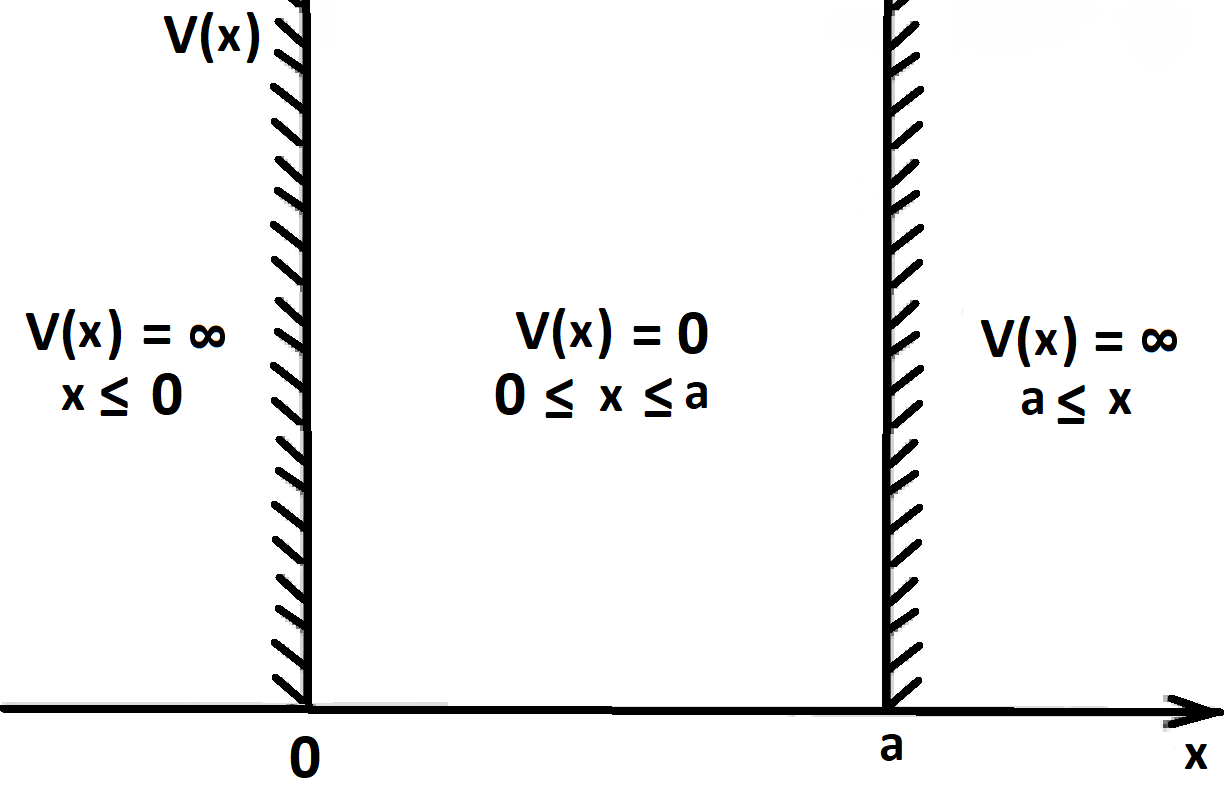
\includegraphics[scale=.65]{infinite_well.png}
\caption{Sonsuz kuyu}
\label{fig:infinite_well}
\end{figure}
%%
Tek boyutlu böyle bir kuyu Schrödinger denklemine,
%%
\begin{equation}
V ( x ) = \left\{
\begin{array} { c l } 
{ \infty } & { \Leftarrow x \leq 0 , x \geq a } \\ 
{ 0 } & { \Leftarrow 0 < x < a } \end{array} 
\right.
\label{eq:infinite_well}
\end{equation}
%%
potansiyelinin konmasıyla tanımlanabilir. Parçacık $0<x<a$ aralığında hapsolduğundan parçacığın dalga fonksiyonu kuyu sınırlarında ve dışında sıfır olmalıdır,
%%
\begin{align*} 
u ( x ) &= 0 \quad x \leq 0 \\ 
u ( x ) &= 0 \quad x \geq a .
\end{align*}
%%
Problemin doğasından ortaya çıkan bu şartlar \emph{sınır şartları} olarak adlandırılır. Kutu dışındaki her yerde dalga fonksiyonu sıfır olduğundan kutunun dışı için Schrödinger denklemi yazılamaz. Kutunun içindeyse $V(x)=0$ olduğundan, birazcık matematiksel düzenlemeyle, Schrödinger denklemi,
%%
\begin{equation}
\frac { d ^ { 2 } u ( x ) } { d x ^ { 2 } } + \frac { 2 m E } { \hbar ^ { 2 } } u ( x ) = 0
\label{eq:infinite_well_schrodinger}
\end{equation}
%%
olarak yazılılır. Eğer parçacığın enerjisi ($E<0$) negatif ise, $\kappa ^ { 2 } = 2 m | E | / \hbar ^ { 2 }$ olmak üzere,
%%
\begin{equation}
\frac { d ^ { 2 } u ( x ) } { d x ^ { 2 } } - \kappa ^ { 2 } u ( x ) = 0
\end{equation}
%%
denklemine ulaşılır. Bu denklemin en genel çözümü $e ^ { - \kappa x }$ ve $e ^ {\kappa x }$ ifadelerinin lineer bir kombinasyonu olur. Elde edilen çözüm $x=0$'da sınır şartlarını sağlasa da $x=a$'da sınır şartlarını sağlamaz. Böylece $E<0$ seçeneği anlamsızlaşır.

Eğer parçacığın enerjisi ($E>0$) pozitif ise,
%%
\begin{equation}
k ^ { 2 } = \frac { 2 m E } { \hbar ^ { 2 } }
\end{equation}
%%
olmak üzere,
%%
\begin{equation}
\frac { d ^ { 2 } u ( x ) } { d x ^ { 2 } } + k ^ { 2 } u ( x ) = 0
\end{equation}
%%
denklemi elde edilir. Bu denklemin en genel çözümlerinden birisi aşağıdaki gibidir.
%%
\begin{equation}
u(x) = A \sin k x + B \cos k x
\end{equation}
%%
$u(0)=0$ sınır şartı gereğince,
\begin{equation*}
u(0) = A\cdot 0 + B = 0
\end{equation*}
olduğundan $B=0$ olur ve birinci sınır şartını sağlayan genel çözüm,
%%
\begin{equation}
u(x) = A \sin k x
\end{equation}
%%
olarak bulunur. Diğer sınır şartına göre $u(a)=0$ olmalıdır, bu şartın sağlanması ancak,
%%
\begin{equation}
k a = n \pi \quad n = 1,2,3 , \ldots
\end{equation}
%%
olması ile mümkündür. Böylece, $E = p^2/2m = (\hbar k)^2/2m$ olduğu da hatırlanırsa parçacığın sahip olabileceği izinli enerji değerlerinin veya yeni adıyla enerji özdeğerlerinin,
%%
\begin{equation}
E _ { n } = \frac { \hbar ^ { 2 } k ^ { 2 } } { 2 m } = \frac { \hbar ^ { 2 } \pi ^ { 2 } n ^ { 2 } } { 2 m a ^ { 2 } } \quad n = 1,2,3 , \ldots
\end{equation}
%%
olacağı açıktır. Özfonksiyonlar ise normalize edildiklerinde $A=\sqrt { \frac { 2 } { a } }$ olacağından,
%%
\begin{equation}
u _ { n } ( x ) = \sqrt { \frac { 2 } { a } } \sin \frac { n \pi x } { a }
\end{equation}
%%
halinde elde edilirler. Çözümlerin ilginç bir sonucu vardır; farklı enerji özdeğerlerine ortaya çıkaran farklı özfonksiyonlar bibrbirlerine \emph{diktir}. Ayrıca birbirine dik olan bu özfonksiyonlar normalize edilmişler ise \emph{ortonormal} özfonksiyonlar olarak adlandırılırlar. Çalıştığımız problemdeki özfonksiyonlar ortonormaldir, aşağıdaki matematiksel işlem süreciyle bu gösterilmiştir.
%%
\begin{align} 
	\int _ { 0 } ^ { a } d x \, u _ { n } ^ { * } ( x ) u _ { m } ( x ) 
	& = \int _ { 0 } ^ { a } d x \frac { 2 } { a } \sin \frac { n \pi x } { a } \sin \frac { m \pi x } { a } \nonumber\\ 
	& = \frac { 1 } { a } \int _ { 0 } ^ { a } d x \left\{ \cos \frac { ( n - m ) \pi x } { a } - \cos \frac { ( n + m ) \pi x } { a } \right\} \nonumber\\ 
&=\left\{
\begin{array} { c l }
{ \frac { \sin ( n - m ) \pi } { ( n - m ) \pi } - \frac { \sin ( n + m ) \pi } { ( n + m ) \pi } = 0 } & { \Leftarrow n \neq m } \\ 
{\frac{1}{a}\left[x-\frac{a}{2 n \pi}\sin(\frac{2n\pi x}{a})\right]_0^a = 1 } & { \Leftarrow n = m} 
\end{array} 
\right.
\end{align}
%%
İntegrallerin herhangi bir $n$ ve $m$ için cevabı yukarıdaki gibidir, $n$ ve $m$ tam sayılar olduklarından integral sonucu aşağıdaki gibi özetlenebilir.
%%
\begin{equation}
\int _ { 0 } ^ { a } d x \, u _ { n } ^ { * } ( x ) u _ { m } ( x )  = \left\{
\begin{array} { c l } 
{ 0 } & { \Leftarrow n \neq m } \\ 
{ 1 } & { \Leftarrow n = m} 
\end{array} 
\right.
\label{eq:orthonormality}
\end{equation}
%%
En son olarak aşağıdaki gibi daha güzel bir şekilde Kronecker-Delta fonksiyonu kullanılarak yazılabilir.
%%
\begin{equation}
\int _ { 0 } ^ { a }  d x \, u _ { n } ^ { * } ( x ) u _ { m } ( x ) = \delta _ { m n }
\end{equation}
%%
Bu son eşitlik \emph{ortonormalite şartı} olarak tanımlanır. Çalıştığımız problemlerde özfonksiyonlar reel olsa da başka problemler için böyle olmak zorunda değildir, bu nedenle yapılan tanımda özfonksiyonun eşleniği ve kendisi bulunmaktadır.

Enerji özdeğer ve özfonksiyon çözümlerinden bazı fiziksel yorumlar çıkarabiliriz.

\begin{enumerate}
	\item En düşük enerji seviyesi durumu $u_1(x)$ özfonksiyonu ile tanımlanır ve parçacığın sahip olduğu enerji \emph{taban durum enerjisi} olarak adlandırılır,
	%%
	\begin{equation}
	E _ { 1 } = \frac { \pi ^ { 2 } \hbar ^ { 2 } } { 2 m a ^ { 2 } }.
	\end{equation}
	%%
	Klasik durumda en düşük enerji seviyesi kinetik ve potansiyel enerjinin sıfır, yani toplam enerjinin sıfır olduğu durumdur. Kuantum fiziğinde ise minimumda olsa bir enerjinin varlığı söz konusudur.
	
	\item $\langle p \rangle$ beklenen değerini bu sistem için hesaplarken  öncelikle özfonksiyonların reel olduğu hatırlanırsa $u^\ast_{ n } = u _ { n }$ olur. Böylece,
	%%
	\begin{equation}
	\begin{aligned} 
	\langle p \rangle 
	& = \int _ { 0 } ^ { a } d x u _ { n } ( x ) \left( - i \hbar \frac { d u _ { n } ( x ) } { d x } \right) 
	= - i \hbar \int _ { 0 } ^ { a } d x \frac { d } { d x } \frac { \left( u _ {n} ( x ) \right) ^ { 2 } } { 2 } \\ 
	& = - \frac { i \hbar } { 2 } \left[ u _ { n } ^ { 2 } ( a ) - u _ { n } ^ { 2 } ( 0 ) \right] = 0 
	\end{aligned}
	\end{equation}
	%%
	sonucuna ulaşılır. $\langle p \rangle = 0$ olması parçacığın $-x$ ve $+x$ yönlerinde eşit miktarda hareket etmiş olması olarak yorumlanabilir.
	
	\item Diğer taraftan $\left\langle p ^ { 2 } \right\rangle$ sıfır olmaz ve herhangi bir $u_n(x)$ özfonksiyonu için,
	%%
	\begin{equation}
	\left\langle p ^ { 2 } \right\rangle = 2 m E _ { n } = \frac { \hbar ^ { 2 } \pi ^ { 2 } n ^ { 2 } } { a ^ { 2 } }
	\end{equation}
	%%
	olarak bulunur.
	
	\begin{figure}
	\begin{minipage}{.48\textwidth}
		\centering
		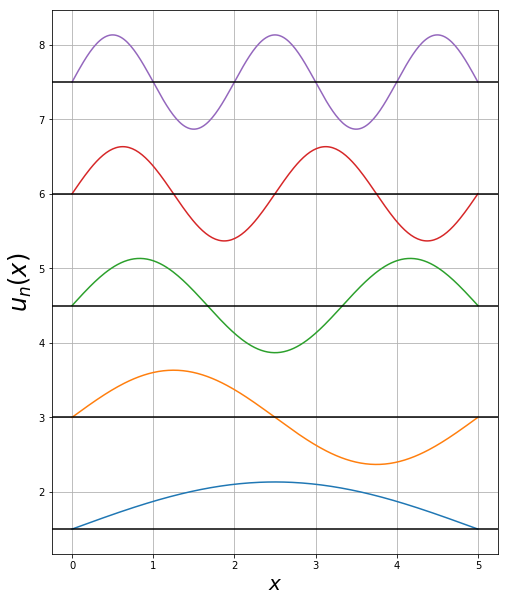
\includegraphics[width=\linewidth]{infinite_well_eigenfunctions.png}
		\caption{Sonsuz kuyudaki parçacığın özfonksiyonları. Dikkat edilirse genlikler sabit ve artan $n$ değerinden bağımsızdır.}
		\label{fig:infinitewell_eigenfunctions}
    \end{minipage}	
    \hspace{12pt}
	\begin{minipage}{.48\textwidth}
	\centering
	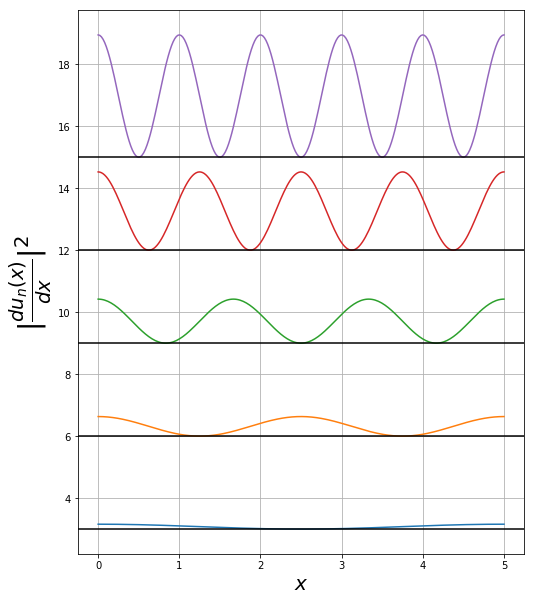
\includegraphics[width=\linewidth]{infinite_well_derivative_of_eigenfunctions.png}
	\caption{Sonsuz kuyudaki parçacığın özfonksiyonlarının türevlerinin kareleri. Dikkat edilirse artan $n$ ile genlikler de büyümektedir.}
	\label{fig:infinitewell_derivative_eigenfunctions}
     \end{minipage}
	\end{figure}
	
	
	\item Düğüm sayısı ($N_D \equiv n-1$) olarak tanımlanabilir, çünkü genellikle sınırlardaki sıfırlar sayılmaz. Bu tanıma göre $n=1$ için $N_D=0$ düğüm varken, $n=2$'de sadece $N_D=1$ düğüm vardır ve bu düğüm tam özfonksiyonun $x=a/2$'de sıfır olduğu yerdir. Düğüm noktası sayısı ($N_D$) arttıkça veya daha üst seviyelere ($n$) çıkıldıkça kinetik enerji artmaktadır. Bunun sebebi aşağıda hesaplanan $\langle K \rangle $ kinetik enerji beklenen değerinden açıkca görülmektedir. Çünkü $\langle K \rangle = E_n$'dir. Ayrıca Şekil \ref{fig:infinitewell_derivative_eigenfunctions}'ten görüleceği üzere integralin iç kısmının genliği $n$ veya $N_D$ arttıkça artmaktadır.
	%%
	\begin{equation}
	\begin{aligned} 
	\langle K \rangle 
	& = \frac { \left\langle p ^ { 2 } \right\rangle } { 2 m } = - \frac { \hbar ^ { 2 } } { 2 m } \int _ { - \infty } ^ { \infty } d x u ^ { * } ( x ) \frac { d ^ { 2 } u ( x ) } { d x ^ { 2 } } \\ 
	& = - \frac { \hbar ^ { 2 } } { 2 m } \int _ { - \infty } ^ { \infty } d x \left\{ \frac { d } { d x } \left( u ^ { * } ( x ) \frac { d u ( x ) } { d x } \right) - \frac { d u ^ { * } ( x ) } { d x } \frac { d u ( x ) } { d x } \right\} \\ 
	& = \frac { \hbar ^ { 2 } } { 2 m } \int _ { - \infty } ^ { \infty } d x \left| \frac { d u ( x ) } { d x } \right| ^ { 2 } \\
	&= \frac { \hbar ^ { 2 } \pi ^ { 2 } n ^ { 2 } } { 2 m a ^ { 2 } }
	\end{aligned}
	\end{equation}
		
	
	\item Şekil \ref{fig:infinitewell_eigenfunctions}'deki özfonksiyonlar arasında ilginç bir davranış gözlenmektedir. Eğer tam orta noktaya ($x=a/2$) bir ayna yerleştirdiğimizi düşünürsek; tek değerli $n=1, 3, 5 \ldots$ özfonksiyonlar simetriktirler, çift değerli $n=2, 4, 6 \ldots$ olanlar ise anti-simetriktirler (yani işaret değiştirmektedirler). Bu simetrinin bir benzerini, 
	%%
	\begin{equation*}
	x \rightarrow x - \frac { a } { 2 }
	\end{equation*}
	%%
	olacak şekilde kuyuyu kaydırarak ve sonra aynayı $x=0$'a taşıyarak da gözleyebiliriz. Böylece, ortaya çıkardığımız bu simetri kullanılarak, sınırları $x=-a/2$ ve $x=a/2$ olan sonsuz kuyu için de çözümler elde edilebilir. Yukarıda yaptığımız değişken dönüşümünü özfonksiyonda da işletirsek,
	%%
	\begin{equation}
	\sin \frac { n \pi x } { a } \rightarrow \sin \left( \frac { n \pi x } { a } - \frac { n \pi } { 2 } \right) = \sin \frac { n \pi x } { a } \cos \frac { n \pi } { 2 } - \cos \frac { n \pi x } { a } \sin \frac { n \pi } { 2 }
	\end{equation}
	%%
	sonucunu elde ederiz. Bu ifadeden anlaşılacağı üzere $x=\pm a/2$ sınırlarına sahip sonsuz kuyu için çift ve tek değerli durumların özfonksiyonları aşağıdaki gibi olacaktır;
	
	%%
	\begin{equation}
	u _ { n } ( x ) = \sqrt { \frac { 2 } { a } } \cos \frac { n \pi x } { a } \quad \text {için } n = 1,3,5 , \dots
	\end{equation}
	%%
	\begin{equation}
	u _ { n } ( x ) = \sqrt { \frac { 2 } { a } } \sin \frac { n \pi x } { a } \quad \text{için } n = 2,4,6, \dots
	\end{equation}
	%%
	Ayrıca, $n = 1,3,5, \dots$ tek sayı şeklindenki kuantum sayılarına karşılık gelen özfonksiyonlar kosinüs fonksiyonları olduklarından $x$'e göre \emph{çift fonksiyon}durlar. Benzeri şekilde $n = 2,4,6, \dots$ çift sayılarına karşılık gelen özfonksiyonlar ise sinüs fonksiyonları olduklarından  $x$'e göre \emph{tek fonksiyon}durlar. Böylece, sonsuz kuyunun ortasında hayal edilen aynaya göre özfonksiyonların neden simetrik ve anti-simetrik davranışlar gösterdikleri daha iyi anlaşılabilir.

	
\end{enumerate}




\subsection{Açılım Varsayımı ve Fiziksel Yorumu }

Fourier teoremine göre $\psi ( 0 ) = 0$ ve $\psi ( a ) = 0$ şartlarını sağlayan herhangi bir sürekli $\psi ( x )$ fonksiyonu,
%%
\begin{equation}
\psi ( x ) = \sum _ { n = 1 } ^ { \infty } C _ { n } \sin \frac { n \pi x } { a }
\end{equation}
%%
formunda yazılabilir. Sonsuz kuyu problemindeki $u_n(x)$ özfonksiyonları sadece bir katsayı farkıyla $\sin n \pi x / a$ ifadesi ile aynıdır. Böylece sonsuz kuyudaki parçacığın toplam dalga fonksiyonunu $u_n(x)$'ler cinsinden,
%%
\begin{equation}
\psi ( x ) = \sum _ { n = 1 } ^ { \infty } A _ { n } u _ { n } ( x )
\end{equation}
%%
olarak elde edeceğimizi iddia edebiliriz. $A_n$ katsayıları ortonormallik şartından aşağıdaki gibi hesaplanabilir:
%%
\begin{equation}
\begin{aligned} \int _ { 0 } ^ { a } d x u _ { m } ^ { * } ( x ) \psi ( x ) & = \int _ { 0 } ^ { a } d x u _ { m } ^ { * } ( x ) \sum _ { n = 1 } ^ { \infty } A _ { n } u _ { n } ( x ) \\ & = \sum _ { n = 1 } ^ { \infty } A _ { n } \int _ { 0 } ^ { a } d x u _ { m } ^ { * } ( x ) u _ { n } ( x ) = \sum _ { n = 1 } ^ { \infty } A _ { n } \delta _ { m n } = A _ { m } \end{aligned}
\end{equation}
%%
olduğundan,
%%
\begin{equation}
A _ { m } = \int _ { 0 } ^ { a } d x u _ { m } ^ { * } ( x ) \psi ( x )
\end{equation}
%%
yazılabilir.

Daha önce serbest parçacığın dalga paketi için yaptığımız tartışmadaki gibi açılım yöntemiyle parçacığın dalga fonksiyonu $\psi(x,t)$'nin zamana bağlı davranışını,
%%
\begin{equation}
\psi ( x , t ) = \psi ( x ) T(t) = \sum A _ { n } u _ { n } ( x ) e ^ { - i E _ { n } t / \hbar }
\end{equation}
%%
olarak yazabiliriz. Hatırlanmalıdır ki, Schrödinger denklemininin kısmi değişkenlere ($x$ ve $t$) ayrıştırılmış halini eşitleyen sabit $E_n$'dir, bu sayede yukarıdaki $e ^ { - i E _ { n } t / \hbar }$ ifadesinin varlığı anlaşılabilir. Bu kısım sadece zaman davranışını izah eden kısmın çözümüdür.

Burada gerçekleştirdiğimiz açılımın vektör analizinde de bir benzeri vardır. $n$ boyutlu bir uzay düşünelim: bu uzayda $\hat i_k$ dik birim vektörlerinin kümesi, özfonksiyonların tam kümesiyle benzer davranışı gösterir. Burada tamlık ile ifade edilmek istenen $n$ boyutlu uzaydaki herhangi bir $\vec a$ vektörü $\hat i_k$ birim vektörlerine açılarak,
%%
\begin{equation}
\vec a = \sum _ { m = 1 } ^ { n } a _ { k } \hat i _ { k }
\end{equation}
%%
şeklinde yazılabilir. Bu birim vektörler dik bir baz oluşturduklarından herhangi iki birim vektör arasında,
%%
\begin{equation}
\hat i  _ { m } \cdot \hat { i } _ { k } = \delta _ { m k }
\end{equation}
%%
bağıntısı vardır. Açılımdaki $a_k$ katsayıları birim vektörler ve $\vec a$ vektörünün iç çarpımı ile,
%%
\begin{equation}
a _ { k } = \hat i _ { k } \cdot \vec a
\end{equation}
%%
bulunabilirler. Böylece anlıyoruz ki; vektörlerdeki iç çarpımın karşılığı özfonksiyonlar durumunda $dx$ üzerinden bir integraldir, ayrıca  $\psi(x)$ ile $\vec a$ ve $u_n(x)$ ile $\hat i_k$ benzer davranışları üstlenmişlerdir.

\subsubsection{Açılım Katsayılarının Fiziksel Yorumu}

$A_n$ katsayılarını yorumlayabilmek için enerjinin beklenen değerini keyfi bir $\psi(x)$ durumunda hesaplayalım. Çalıştığımız örnekte, kuyu içinde $H=p^2/2m$, kuyu dışında $\psi(x)=0$ ve
%%
\begin{equation}
H u _ { n } ( x ) = E _ { n } u _ { n } ( x )
\end{equation}
%%
olduğuna göre,
%%
\begin{equation}
\begin{aligned} 
\langle H \rangle = \int _ { 0 } ^ { a } d x \psi ^ { * } ( x ) H \psi ( x ) 
& = \int _ { 0 } ^ { a } d x \psi ^ { * } ( x ) H \sum _ { n } A _ { n } u _ { n } ( x ) \\ 
& = \sum _ { n } A _ { n } \int^ { a }_{ 0 } d x \psi ^ { * } ( x ) E _ { n } u _ { n } ( x ) \\ 
& = \sum _ { n } E _ { n } \left| A _ { n } \right| ^ { 2 } 
\end{aligned}
\end{equation}
%%
sonucuna ulaşırız. Ayrıca,
%%
\begin{equation}
\int _ { 0 } ^ { a } d x \psi ^ { * } ( x ) \psi ( x ) = 1
\end{equation}
%%
olduğundan,
%%
\begin{equation}
\int _ { 0 } ^ { a } d x \psi ^ { * } ( x ) \sum _ { n } A _ { n } u _ { n } ( x ) 
= \sum _ { n } A _ { n } A _ { n } ^ { * } 
= \sum _ { n } \left| A _ { n } \right| ^ { 2 } = 1
\end{equation}
%%
olur. $|A_n|^2$'yi anlamak için her bir enerji ölçümünün sadece bir enerji özdeğeri ortaya çıkaracağını kabul etmeliyiz. Bu önerme Bohr'un atom modelinde durağan durumlar için, üstü kapalı da olsa, yapılmıştır. Önermeyi kuantum mekaniğine taşırsak; ölçülen bir enerji enerji operatörünün özdeğerlerinden birine karşılık gelir. Bu durumda ortalama enerji ölçümü,
%%
\begin{equation}
E _ {ort} = \langle \hat H \rangle = \sum _ { n } E _ { n } P _ { n }
\end{equation}
%%
olur. Burada $P_n$ elde edilen her bir ölçümde $E_n$ enerji özdeğerini ölçme olasılığıdır. Olasılıkların toplamı,
%%
\begin{equation}
\sum _ { n } P _ { n } = 1
\end{equation}
%%
olacaktır. Bu sonuçlardan,
%%
\begin{equation}
P_n = |A_n|^2
\end{equation}
%%
olduğu ve \emph{`` $|A_n|^2$ yapılan bir enerji ölçümünde $\psi(x)$ durumunun $E_n$ enerji özdeğeri üretme olasılığıdır"} yorumlarını yapabiliriz. Daha önce de gösterdiğimiz üzere $A_n$ katsayıları,
%%
\begin{equation}
A _ { n } = \int _ { 0 } ^ { a } d x u _ { n } ^ { * } ( x ) \psi ( x )
\end{equation}
%%
ile elde edilirler.

\subsection{Serbest Parçacık ve Momentum Özfonksiyonu}

Enerji operatörü $\hat H$ dışında da özfonksiyon ve özdeğerleri olan operatörler vardır. Bunlardan birisi $\hat p$ \emph{momenum operatörüdür}: bu operatör dalga fonksiyonuna işletildiğinde,
%%
\begin{equation}
\hat p u _ { p } ( x ) = p u _ { p } ( x ), \quad \hat p \equiv \frac{\hbar}{i} \frac{d}{dx}
\end{equation}
%%
özfonskiyon ve özdeğerleri ortaya çıkar. Operatörün açık hali yazılır ve dalga fonksiyonuna uygulanırsa,
%%
\begin{equation}
\frac { d u _ { p } ( x ) } { d x } = \frac { i p } { \hbar } u _ { p } ( x )
\end{equation}
%%
birinci dereceden adi bir diferansiyel denklem ortaya çıkar. Bu denklemin genel çözümü,
%%
\begin{equation}
u _ { p } ( x ) = C e ^ { i p x / \hbar }
\end{equation}
%%
şeklindedir. Burada $C$ belirsiz bir sabittir ve normalizasyon ile hesaplanabilir. $p$ özdeğeri reel değerlidir böylece $u_p(x)$ özfonksionu $x \rightarrow \pm \infty$ durumunda patlamaz ve sonlu kalır. Serbest bir parçacık için $\hat p$ operatörünün davranışını incelediğimizden, p özdeğeri kesikli değerler değil sürekli değerler alır. Diğer bir ifadeyle $\hat p$'nin sürekli bir spektrumu vardır, denebilir. Enerji özfonksiyonları gibi momentum özfonksiyonları da,
%%
\begin{equation}
\int _ { - \infty } ^ { \infty } d x u _ { p ^ { \prime } } ^ { * } ( x ) u _ { p } ( x ) = \delta \left( p - p ^ { \prime } \right)
 = \left\{
\begin{array} { c l } 
{ 0 } & { \Leftarrow p \neq p^\prime } \\ 
{ 1 } & { \Leftarrow p   =  p^\prime} 
\end{array} 
\right.
\end{equation}
%%
yukarıda verilen ortonormalite (dik ve birim olma) şartına uyuyorlarsa,

\begin{equation}
\begin{aligned} 
\int _ { - \infty } ^ { \infty } d x u _ { p ^ { \prime } } ^ { * } ( x ) u _ { p } ( x ) 
& = | C | ^ { 2 } \int _ { - \infty } ^ { \infty } d x e ^ { i \left( p - p ^ { \prime } \right) x / \hbar } \\ 
& = 2 \pi | C | ^ { 2 } \hbar \delta \left( p - p ^ { \prime } \right) 
\end{aligned}
\end{equation}
%%
olacaktır.İntegralin sonucu $p=p^\prime$ için $1$ olacağından $C$'nin değeri de bulunmuş olur. Böylece momentum özfonksiyonu,
%%
\begin{equation}
u _ { p } ( x ) = \frac { 1 } { \sqrt { 2 \pi \hbar } } e ^ { i p x / \hbar }
\end{equation}
%%
olarak bulunur. Enerji özfonksiyonolarının tam bir setiyle seriye açtığımız $\psi(x)$'i momentum özfonksiyonlarının tam bir setiyle de seriye açabiliriz. Tek fark enerji özdeğerleri kesikli iken, momentum özdeğerleri süreklidir. Eğer momentum özdeğerleri kesikli olsaydı, $\psi(x)$
%%
\begin{equation}
\psi ( x ) = \sum _ { n = 1 } ^ { \infty } A _ { p_n } u _ {p_ n } ( x )
\end{equation}
%%
ifadesine benzer şekilde kesikli özfonksiyonların açılımı şeklinde yazılabilirdi. Fakat $\hat p$ sürekli bir spektruma sahip olduğundan,
%%
\begin{equation}
\psi ( x )  
= \int _ { - \infty } ^ { \infty } d p \phi ( p ) u_p(x)
= \int _ { - \infty } ^ { \infty } d p \phi ( p ) \frac { e ^ { i p x /\hbar } } { \sqrt { 2 \pi \hbar } }
\label{eq:psi_x_complete_set_expansion}
\end{equation}
%%
$\psi(x)$ $u_p(x)$ özfonksiyonlarının tam bir setiyle yukarıdaki gibi yazılmalıdır. Burada,
%%
\begin{align*}
\phi(p) &\leftrightarrow A_n \\
u_p(x)  &\leftrightarrow u_n(x) 
\end{align*}
%%
benzerliklerinin varlığına dikkat edilmelidir. $A_n$'lerin bulunmasına benzer şekide $\phi(p)$'lerde
%%
\begin{equation}
\phi ( p )
= \int _ { - \infty } ^ { \infty } d x u^\ast_p(x)  \psi ( x )
= \int _ { - \infty } ^ { \infty } d x \left( \frac { e ^ { i p x / \hbar } } { \sqrt { 2 \pi \hbar } } \right) ^ { * } \psi ( x )
\label{eq:phi_p_complete_set_expansion}
\end{equation}
%%
integraliyle (iç çarpımıyla) hesaplanabilirler. Aslında Denk. \ref{eq:psi_x_complete_set_expansion} ve \ref{eq:phi_p_complete_set_expansion} karşılaştırmalı olarak incelenirse; Denk. \ref{eq:psi_x_complete_set_expansion}'te $\psi(x)$'in momentum özfonksiyonlarının ve $\phi(p)$ katsayılarının bir açılımı olarak, Denk. \ref{eq:phi_p_complete_set_expansion}'da ise $\phi(p)$'nin momentum özfonksiyonlarının ve $\psi(x)$ katsayılarının bir açılımı olarak yazıldığı düşünülebilir. Böylece daha önce de bahsettiğimiz gibi $\psi(x)$ konum uzayındaki dalga fonksiyonu iken, $\phi(p)$ momentum uzayındaki dalga fonksiyonudur önermesi daha kuvvetli bir dayanak kazanmış olur.

\subsubsection{Serbest Parçacık Dalga Fonksiyonunun Normalizasyonu}

Serbest parçacık durumunu incelemeye devam edelim. Serbest parçacık için potansiyel $V(x)$ heryerde sıfır olacaktır, bu nedenle Hamiltonyen işlemcisi sadece kinetik enerji kısmını içerecek şekilde,
%%
\begin{equation}
\frac { d ^ { 2 } u ( x ) } { d x ^ { 2 } } + \frac { 2 m E } { \hbar ^ { 2 } } u ( x ) = \frac { d ^ { 2 } u ( x ) } { d x ^ { 2 } } + k ^ { 2 } u ( x ) = 0
\label{eq:freeParticle_schEq}
\end{equation}
%%
olarak yazılır. Bu diferansiyel denklemin çözümleri $e ^ { i k x }$, $e ^ { - i k x }$ veya $\sin kx$, $\cos kx$ fonksiyonlarının lineer kombinasyonları olacaktır. Örneğin, $+x$ yönünde ilerleyen bir parçacık için
%%
\begin{equation}
\psi(x,t) = u(x) T(t) = A e ^ { i k x -\omega t}
\end{equation}
%%
şeklinde bir serbest dalga fonksiyonu önerilebilir. Zamandan bağımsız Schrödinger denkleminin çözümü ise,
%%
\begin{equation}
u(x) = A e ^ { i k x }
\end{equation}
%%
olacaktır. Fakat bu çözümün problemi karesi integrallenebilir olmamasıdır.
%%
\begin{align}
\int _ { - \infty } ^ { \infty } d x \left|u(x) \right| ^ { 2 } 
&= \int _ { - \infty } ^ { \infty } d x \left|A e ^ { i k x } \right|^2 \nonumber\\
&= \int _ { - \infty } ^ { \infty } d x A^2 \left|e ^ { i k x } \right|^2
= \int _ { - \infty } ^ { \infty } d x A^2 \nonumber\\
&= A^2 x\bigg|_{-\infty}^\infty
\end{align}
%%
Çünkü yukarıdaki işlemlerin sonucundan anlaşılacağı üzere integral ıraksar (patlar). 

Bu sonuç, bir örnekle şöyle yorumlanabilir: Bir elektron tabancasından çıkan elektron demetinin momentumu çok iyi bilindiğinden ($\Delta p \rightarrow 0$), Heisenberg'in belirsizlik ilkesine göre, konumu hakkındaki bilgi tamamen kaybolmuştur ($\Delta x \rightarrow \infty$). Diğer bir ifadeyle $|u(x)|^2 dx = A^2 dx$ parçacığın $dx$ ve $x+dx$ aralığında bulunma olasılığı bütün uzayda aynı değere sahiptir. 
Böyle bir durumu fiziksel olarak kabul etmek pek mümkün değildir. Çünkü elektron tabancasından çıkan elektron demetinin (veya bir başka parçacık hızlandırıcıdan çıkan parçacık demetinin) boyu bilinmektedir. Hızlandırılan parçacık ilk defa tabancadan çıktığında bu demet için de bir yerde olmalıdır. Bu nedenle parçacığın serbest olma özelliğini kaybetmeden parçacığın konumunu yerelleştirebilecek normalizasyon yöntemlerine ihtiyaç duyulur. Dolayısıyla bu tür sistemlerin dalga fonksiyonlarını normalize etmenin farklı yolları önerilmiştir.
%%
\begin{enumerate}
	\item İlk yöntem sonsuz kuyu sınırları $x=\pm a/2$'yi çok genişletmek ve çok daha geniş bir kuyu elde etmek. Fakat ne kadar genişletilse de $\bf e ^ { \pm i k x }$ şeklindeki dalga fonksiyonları sınırlarda yok (sıfır) olmayacaktır. Bu nedenle $\psi (x=\pm a / 2 ) = 0$ sınır şartı değiştirilerek,
	%%
	\begin{equation}
	\psi ( x-a/2) = \psi ( x + a/2 )
	\end{equation}
	%%
	şeklinde yeniden tanımlanır. Yeni tanımlanan bu şart, dalga fonksiyonunun, parçacık serbest olduğu ve her yerde aynı olasılıkla bulunabileceği için, $x=-a/2$ ve $x=+a/2$'de sürekli olmasının gerekliliğinden ortaya çıkar. Böylece,
    %%
	\begin{align*}
	e ^ { i k (x-a/2) } &= e ^ { i k (x+a/2) }\\
	e ^ { i k x}	e ^ { -i k a/2}  &= e ^ { i k x } 	e ^ { i k a/2} \\
	e ^ { i k a} &= 1
	\end{align*}
	%%
	sonucu ortaya çıkar. Genişletilmiş kuyudaki bu yeni sınır şartına uyan dalga için $k~=~2 n \pi / a$ veya $p = 2 \hbar n \pi / a$ olur. Burada $a$ kuyu genişliği ve $n=1,2,3, \ldots$ bir tam sayıdır. Serbest parçacık için momentum herhangi bir değerde olabilir. Bu nedenle $a$ ne kadar genişletilirse parçacığın momentumunu verecek olan $n$ değeri de buna göre büyütülmelidir. Genişletilmiş bu kuyuda artık,
	%%
	\begin{equation}
	A ^ { 2 } \int _ { -a/2 } ^ { a/2 } d x \left| e ^ { i k x } \right| ^ { 2 } = A ^ { 2 } a = 1
	\end{equation}
	%%
	normalizasyonu yapılabilir. Böylece serbest parçacığı temsil eden düzlem dalgalar,
	%%
	\begin{equation}
	u(x) = \frac{1}{\sqrt{a}} e ^ { \pm i k x }
	\end{equation}
	%%
	şeklinde normalize edilmiş olarak yazılabilirler.
	
	
	\item Elektron tabancasından çıkan elektron örneğiyle devam edersek, momentumu çok iyi bilindiğinden momentum uzayında,
	%%
	\begin{equation}
	\phi ( p ) = \sqrt { 2 \pi \hbar } \delta ( p - p^\prime )
	\end{equation}
	%%
	şeklinde bir dalga paketi fonksiyonu önerebiliriz. Bu dalga fonksiyonu sadece $p=p^\prime$ iken sıfırdan farklı diğer durumlarda sıfırdır, böylece momentumun değeri kesin olarak bilinmiş olmaktadır.
	Önerdiğimiz bu dalga paketi ile,
	%%
	\begin{equation}
	u _ { p } ( x ) = \frac { 1 } { \sqrt { 2 \pi \hbar } } e ^ { i p x / \hbar }
	\label{eq:free_particle_wf}
	\end{equation}
	%%
	olarak tanımlı serbest parçacık momentum özfonksiyonunu beraber kullanarak, serbest parçacığın $\psi(x)$ dalga fonksiyonunu,
	%%
	\begin{align}
	\psi ( x )  
	&= \int _ { - \infty } ^ { \infty } d p \phi ( p ) u_p(x)
	= \int _ { - \infty } ^ { \infty } d p  \{\sqrt { 2 \pi \hbar } \delta ( p - p^\prime )\} \frac { e ^ { i p x /\hbar } } { \sqrt { 2 \pi \hbar } }\\
	&= e ^ { i p x /\hbar } =  e ^ { i k x }
	\end{align}
	%%
	şeklinde dalga paketi olarak yazabiliriz. Bu normalizasyon yöntemi \emph{Dirac normalizasyonu} olarak adlandırlır. Bir önceki normalizasyondaki gibi bir sonuç elde etmek için Dirac delta gibi çok keskin bir dalga paketi yerine yine keskin ama her noktada tanımlı bir dalga paketi tercih edilebilir. Böylece gerçek fiziksel demet daha iyi temsil edilmiş olur. Buradaki momentum dalga paketi fonksiyonu çok keskin olduğundan $\Delta p = 0$'dir, fakat Heisenberg'in belirsizlik ilkesi gereği, $\Delta x \rightarrow \infty$ olur.
    % REF: http://fisica.ugto.mx/~supercuerdas/miembros/QM/qm4.pdf)
	%%
	\begin{figure}[hbtp]	
	\begin{minipage}{.45\textwidth}
	\centering
	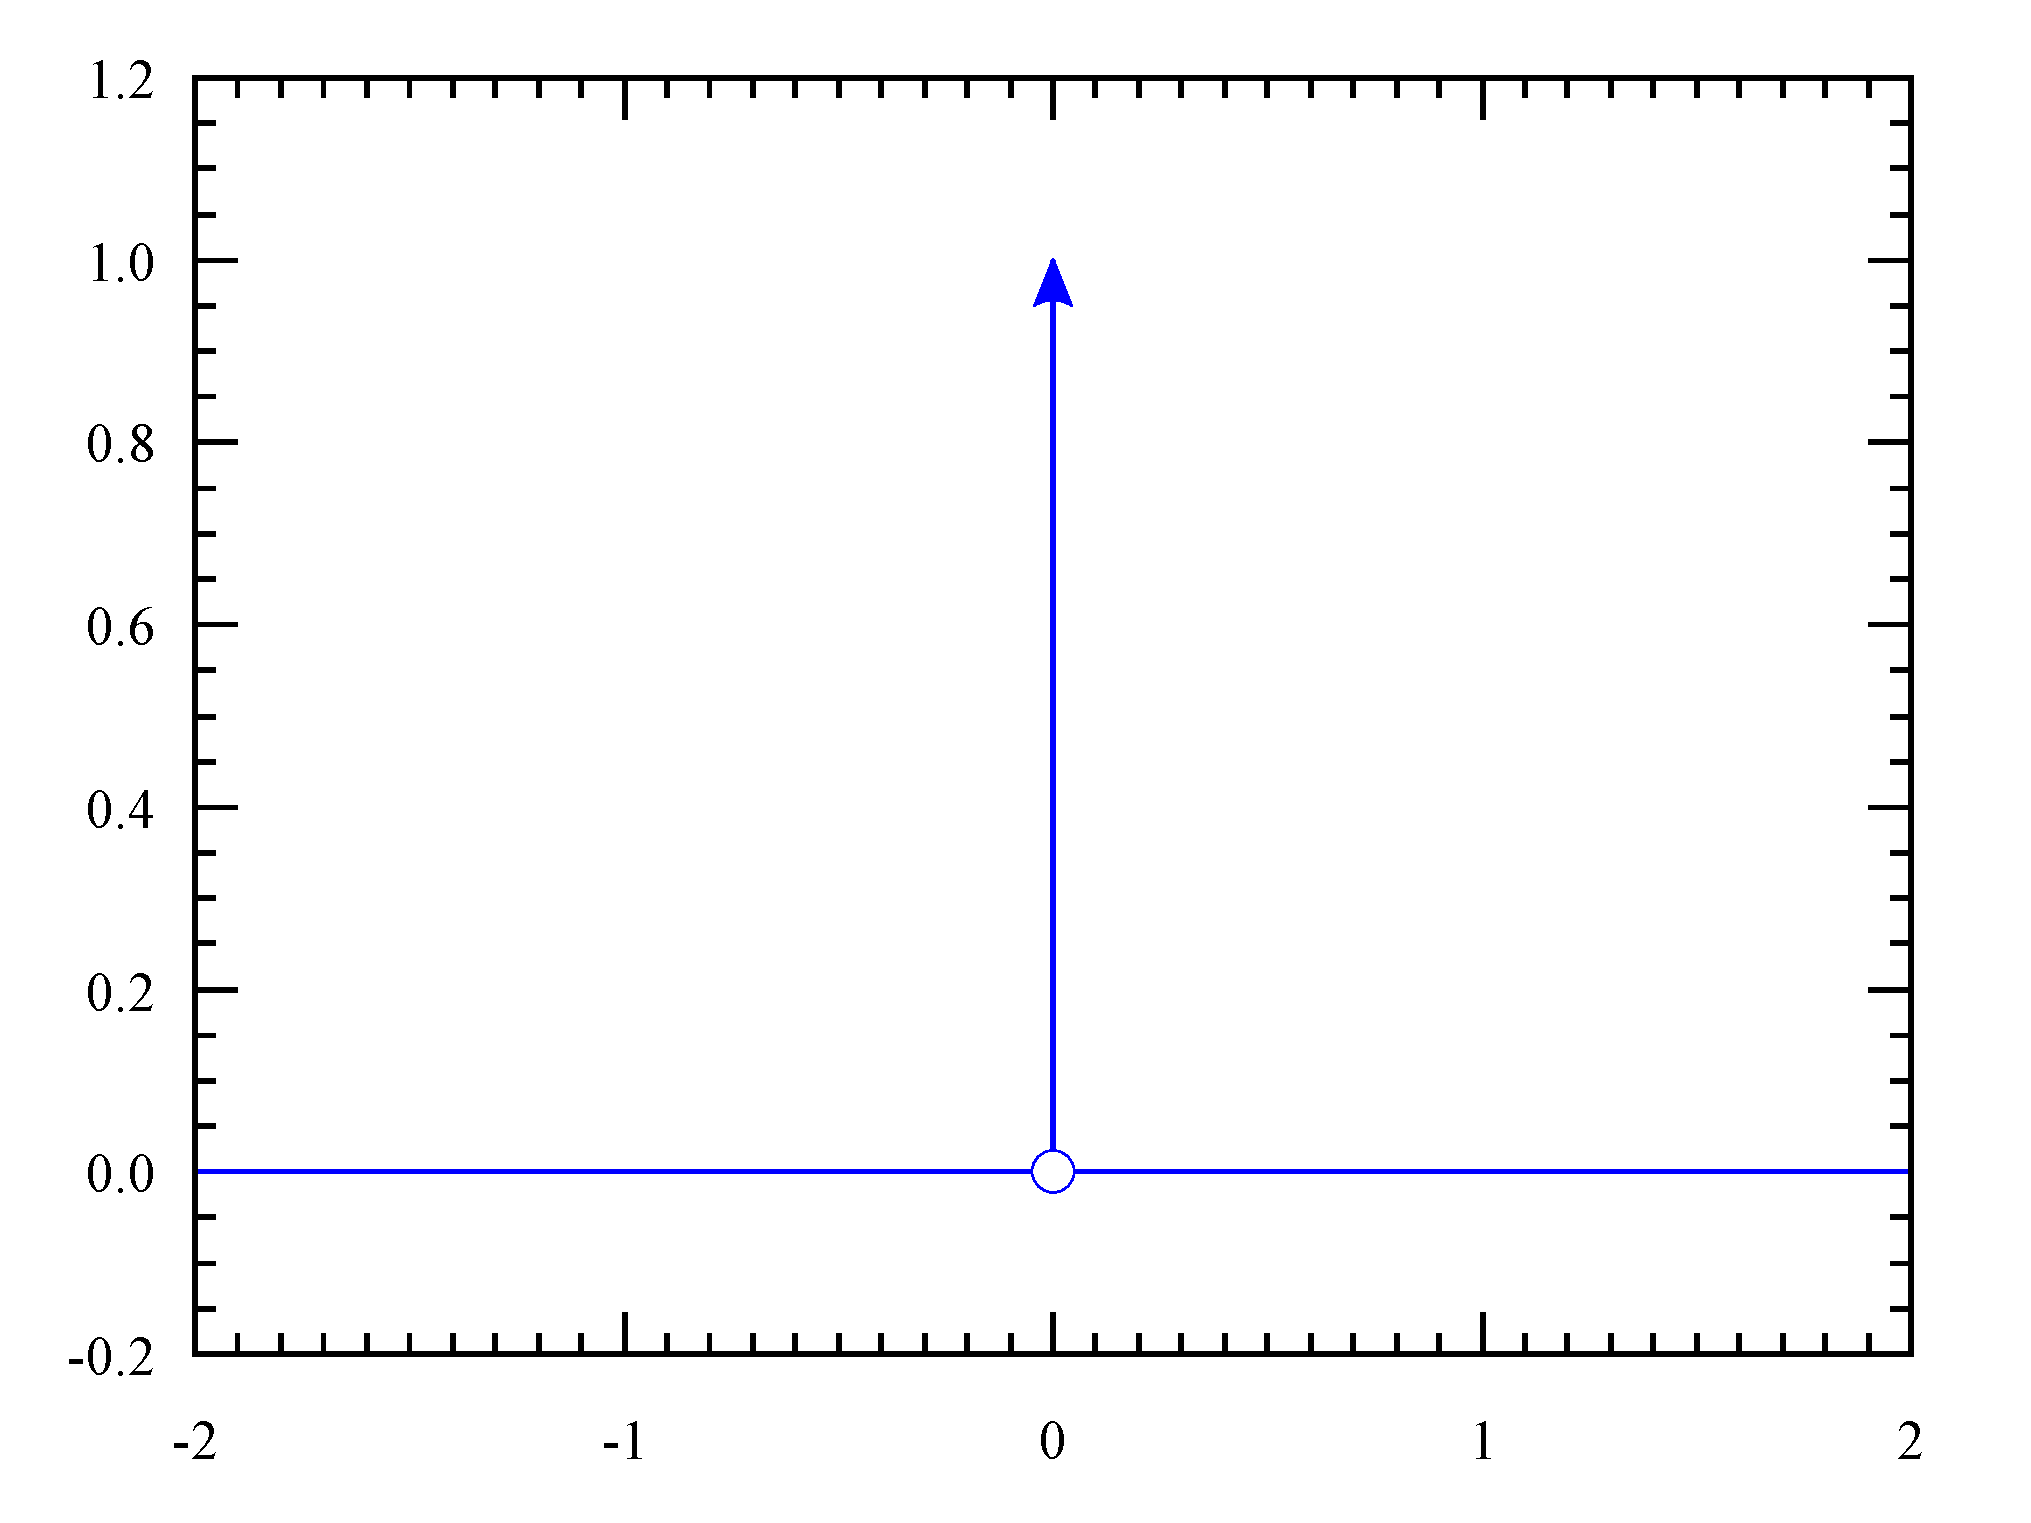
\includegraphics[width=.9\linewidth]{Dirac_distribution_PDF.pdf}
	\caption{Dirac dağılımı.}
	\label{fig:diracdistribution}
	\end{minipage}
    %%
	\begin{minipage}{.10\textwidth}
		\hspace{12pt}
	\end{minipage}
	\begin{minipage}{.45\textwidth}
	\centering
	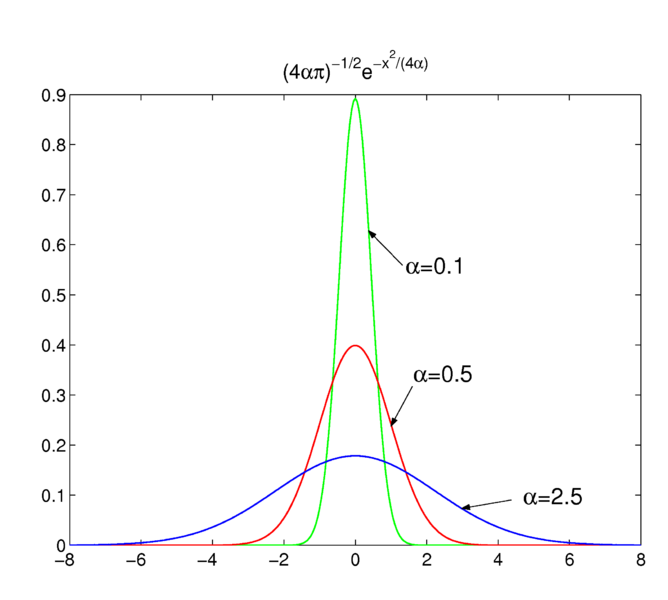
\includegraphics[width=.7\linewidth]{Dirac_delta_gaussian.png}
	\caption{$\alpha \rightarrow 0$ için Dirac dağılımına yaklaşan bir gausyen fonksiyon.}
	\label{fig:diracdistribution1}
    \end{minipage}
    \end{figure}			
	%%
	$\psi(x)$'i daha gerçekçi ve normalize edilebilir hale getirmek için dirac delta fonksiyonu yerine Şekil \ref{fig:diracdistribution1}'teki gibi bir gausyen fonksiyon seçilebilir. Böylece $q=p-p^\prime$ olmak üzere $\psi(x)$ için,
    %%
	\begin{align}
	\psi ( x )  
	&= e ^ { i p^\prime x /\hbar }  \int _ { - \infty } ^ { \infty } d q  \delta ( q )  e ^ { i q x /\hbar }
	\end{align}
	%%
	dalga paketi yazılabilir. Bu dalga paketi çok yavaş değişen ve ilgilenilen bölgede (örneğin demet uzunluğu) neredeyse sabit olan bir dağılım olacaktır. Böylece ıraksamayan, normalize edilebilen daha gerçekçi bir serbest dalga yazılmış olur.
	
	\item Serbest parçacık dalga fonksiyonunun normalizasyonun ıraksamasına sebep olan parçacığın, sonsuz kuyuda olduğu gibi, uzayda herhangi bir yere hapsedilmemiş olmasından kaynaklanmaktadır. Eğer parçacığın sınırlı bir bölgede nerede olduğu sorusunun cevabını aramayı bırakırsak böyle bir sorun da ortaya çıkmamış olur. Bunun yerine olasılık akımı veya akısı ile ilgilenirsek,
	%%
	\begin{equation}
	j ( x ) = \frac { \hbar } { 2 i m } \left[ \psi^\ast ( x ) \frac { d \psi ( x ) } { d x } - \frac { d \psi ^ { \ast } ( x ) } { d x } \psi ( x ) \right]
	\end{equation}
	%%
	normalizasyon problemini daha rahat aşabiliriz. Yukarıdaki tanımına göre $C e ^ {\pm i p x / \hbar }$ gibi bir serbest dalga fonksiyonu için akı $\pm | C | ^ { 2 } p / m$ olur. Olasılık yoğunluğu ve dalga fonksiyonu arasındaki bağıntı hatırlanırsa,
	%%
	\begin{equation}
	P(x) dx = |\psi(x)|^2 dx = |C|^2 dx \quad \Rightarrow \quad [|C|^2]\equiv 1/m
	\end{equation}
	%%
	serbest parçacığın düzlem dalgası için $|C|^2$'nin bir boyutta \emph{1 parçacık/m} kadarlık bir parçacık olasılık yoğunluğunu tanımladığı ortaya çıkar. Böylece $[\pm | C | ^ { 2 } p / m] \equiv 1/s$ olacağı açıktır. Sonuçta bir boyutlu olasılık akısı ile birim uzunluktan ve birim zamanda geçebilecek parçacık olasılığı hesaplanmış olur. Bu sonuca göre, normalize etmeye çalıştığımız serbest parçacık dalga fonksiyonu (Denk. 	\ref{eq:free_particle_wf}) $|C|^2 = 1 / 2 \pi \hbar$~(1/metre) yoğunluklu bir parçacık demetini temsil etmektedir.
	%%
	%% Unit of a wavefunction read from the following link
	%% https://www.researchgate.net/post/Does_wave_function_in_Quantum_mechanics_have_a_unit
	
	Üç boyutlu durumdaysa serbest parçacık dalga fonksiyonu,
	%%
	\begin{equation}
	u _ { p } ( \vec{ r } ) = C e ^ { i \vec { p } \cdot \vec { r } / \hbar }
	\end{equation}
	%%
	halini alır ve akı yine $|C|^2 p/m$ olur. Fakat birimi $\frac{1/s}{m^2}$ olur, çünkü $\vec p$ momentum vektörüne dik bir birim alandan geçen ve birim hacim başına $|C|^2$ kadar yoğunluğa sahip parçacık demetini temsil eder.
	%%
	\begin{figure}[hbtp]
		\centering
		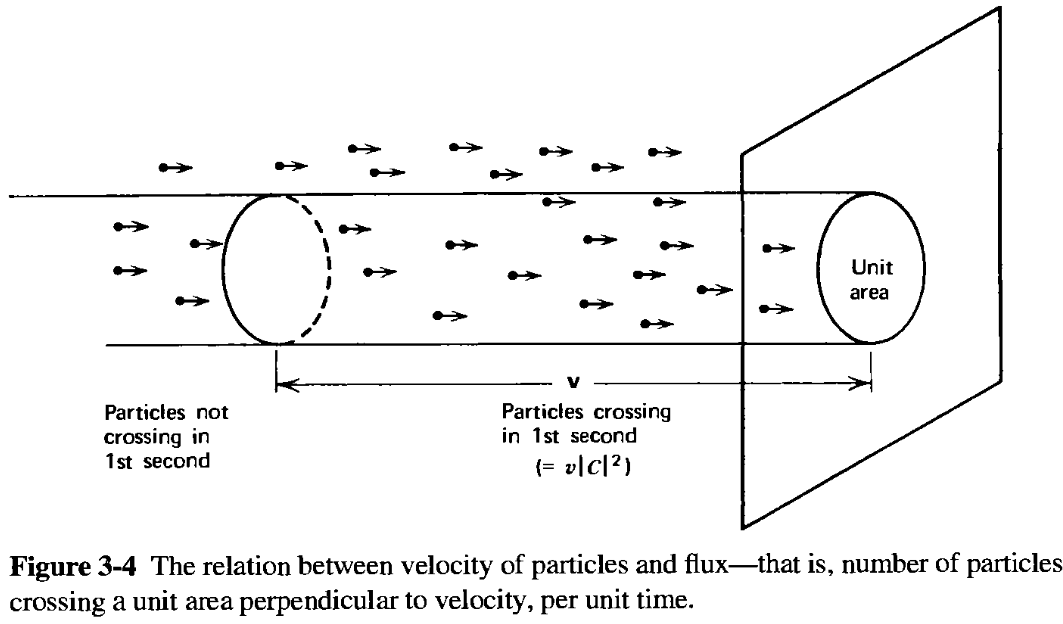
\includegraphics[width=0.5\linewidth]{figurler/normalization_and_probab_flux}
		\caption{\YAZILACAK, değişecek veya silinecek...}
		\label{fig:normalizationandprobabflux}
	\end{figure}
	
	
	
\end{enumerate}

\subsubsection{Yozlaşmış (Dejenere) Durumlar}

Enerji özdeğeri denkleminin (Denk. \ref{eq:freeParticle_schEq}), $u_1(x) = e^{i k x}$ ve $u_2(x) = e^{-i k x}$  olmak üzere birbirinden bağımsız iki çözümü vardır. Benzer şekilde bu denklemin reel çözümleri $u_1(x) = \cos(kx)$ ve $u_2(x) = \sin(kx)$'te bağımsız çözümlerdir. Bu çözümlerden hangi $u_1(x)$, $u_2(x)$ ikilisi seçilirse seçilsin, sonsuz kuyudaki parçacık probleminden farklı olarak, her ikiside aynı enerji özdeğerine sahip olacaktır. Serbest parçacık için Hamiltonyen işlemcisi her iki çözüme uygulandığında aşağıdaki sonuca ulaşılacağı rahatça gösterilebilir.

\begin{equation}
-\frac{ \hbar ^ { 2 } } { 2 m} \frac { d ^ { 2 } u_1 ( x ) } { d x ^ { 2 } }  =  E u_1 ( x ), \quad\quad
-\frac{ \hbar ^ { 2 } } { 2 m} \frac { d ^ { 2 } u_2 ( x ) } { d x ^ { 2 } }  =  E u_2 ( x )
\end{equation}

Birden çok bağımsız özfonksiyonun bir hermityen işlemcinin aynı özdeğerine karşılık geldikleri durumlarla karşılaşılabilir, bu tür durumlara yozlaşmış (dejenere) durumlar denir.

Her iki dejenere özfonksiyon ikilisi de birbirlerine diktir (ortogonaldir). Aşağıdaki integraller $k\neq0$ ve $a\rightarrow\infty$ (serbest parçacık olması için $a$ sonsuza gitmelidir) olmak üzere dejenere özfonksiyonların birbirlerine dik olduklarının kanıtlarıdır.
%%
\begin{align}
	{\int\limits_{-a}^{a} d x\left(\frac{1}{\sqrt a}e^{-i k x}\right)^{*} \left(\frac{1}{\sqrt a}e^{i k x}\right)=0} \text{ \quad ve \quad }
	{\int\limits_{-a}^{a} d x \sin k x \cos k x=0}
\end{align}
%%
Aynı enerjiye $E=\hbar^{2} k^{2} / 2 m$ karşılık gelen kaç tane dejenere durum (özfonksiyon) olursa olsun, bu özfonksiyonlar \emph{farklı enerjilere} ait özfonksiyonlara daima diktirler. 

Enerji özdeğerine göre dejenere olan özfonksiyonlar başka bir operatörün de özfonksiyonları olabilirler ve bu diğer operatöre göre dejenere olmayabilirler. Örneğin momentum işlemcisi ($\hat p$) için $e^{\pm i k x}$ özfonksiyonları dejenere değildirler.
%%
\begin{align}
\hat p e^{i k x}&=\frac{\hbar}{i} \frac{d}{d x} e^{i k x}=\hbar k e^{i k x} \nonumber\\
\hat p e^{- i k x}&=\frac{\hbar}{i} \frac{d}{d x} e^{- i k x}=- \hbar k e^{- i k x}
\end{align}
%%
$p=\hbar k$ olmak üzere $\pm p$ her iki özfonksiyon için iki farklı özdeğer mevcuttur.

Eğer $\cos(kx)$ ve $\sin(kx)$ çiftini inceleyecek olsaydık, bu iki özfonksiyonu birbirinden ayırt edecek olan momentum işlemcisi olmazdı. Çünkü bu özfonksiyonlar momentum işlemcisinin özfonksiyonları değildirler. Bu özfonksiyonları ayırt etmemizi sağlayacak başka bir kavram vardır: $x$'e göre $\cos(kx)$ çift ve $\sin(kx)$ tek fonksiyondur. \emph{Çift} veya \emph{tek} olma özdeğerleri olarak adlandırabileceğimiz bu durumları $\hat P$ parite işlemcisi olarak adlandırcağımız işlemci vermektedir.
%%
\begin{align}
\hat P \cos( k x)&= \cos( - k x) = +1 \cos(k x)  \nonumber\\
\hat P \sin( k x)&= \sin( - k x) = -1 \sin(k x)
\end{align}
%%
Yukarıdaki işlemlerin sonucuna göre her iki özfonksiyon için $\hat P$'nin $\pm 1$ şeklinde farklı iki özdeğeri mevcuttur. Buna göre $\cos(kx)$ \emph{çift parite} ve $\sin(kx)$ \emph{tek parite} özdeğerlidir.


\subsubsection{Parite}

%% watch: https://www.youtube.com/watch?v=yArprk0q9eE

% READ FOLLOWING!
% http://www.physics.udel.edu/~msafrono/424-2011/Lecture%209final.pdf
% http://fisica.ugto.mx/~supercuerdas/miembros/QM/qm4.pdf
% http://folk.uio.no/trondson/freeparticle.pdf
% https://physics.stackexchange.com/questions/165373/normalizing-the-solution-to-free-particle-schr%C3%B6dinger-equation


Bir serbest parçacığın veya ($-a/2$ ve $+a/2$ sınırlı ve  $x=0$ etrafında simetrik olan) bir sonsuz kuyu içindeki parçacığın $\sin(kx)$ ve $\cos(kx)$ özfonksiyonlarıyla tanımlanabildiğini gördük. Bu özfonksiyonlar $x \rightarrow -x$ dönüşümü altında \emph{tek} veya \emph{çift} fonksiyonlardır.
Sonsuz kuyu içeresindeki örneği düşünecek olursak; bu sistemin (taban seviyesindeki) ilk durumu $\psi(x)$ $x$'e göre çifttir. Bunun anlamı $n=1,3,5,\ldots$ olmak üzere $\psi(x)$,
%%
\begin{equation}
\psi(x)=\sum_{n} A_{n} \sqrt{\frac{2}{a}} \cos \frac{n \pi x}{a}
\end{equation}
%%
şeklinde olmalıdır. Zamana göre değişimi ise,
%%
\begin{equation}
\psi(x, t)=\sum_{n} A_{n} \sqrt{\frac{2}{a}} \cos \frac{n \pi x}{a} e^{-i E_{n} t / \hbar}
\end{equation}
%%
olacaktır. Zamana bağlı dalga fonksiyonunun da $x$'e göre hala \emph{çift} kalacağı açıktır. Aynı durum başlangıçta \emph{tek} fonksiyon olan dalga fonksiyonları için de geçerlidir. Böylece $x=0$ civarında simetrik olan bu sistem için \emph{çiftlik} veya \emph{teklik} zamandan bağımsız bir özelliktir. Bu durumda \emph{çift} ve \emph{tek} olma durumlarına bu \emph{hareketin sabitleri}dir, denebilir. 

Fizikte herhangi bir harekete ait sabit daima önemlidir, çünkü sabitin temsil ettiği ilgili niceliğin zamanla (veya ilgili olduğu boyutla; zaman, konum, momentum vb.) korunduğunu gösterir. Bu tür sabitleri formülleştirmek faydalıdır; \emph{çift} veya \emph{tek} olma durumunu parite işlemcisi $\hat P$ ile formülleştirebiliriz. İşlemcinin görevi basitçe $x\rightarrow -x$ yansımasını gerçekleştirmektir. Parite işlemcisi herhangi bir dalga fonksiyonuna uygulandığına,
%%
\begin{align}
\hat P \psi(x)=\psi(-x)
\end{align}
%%
işlemini gerçekleştirir. Çift ve tek fonksiyonlar için bu işlemin sonucu,
%%
\begin{align}
\hat P \psi^{(+)}(x)=\psi^{(+)}(x)
\quad \text{ ve } \quad \hat P \psi^{(-)}(x)=-\psi^{(-)}(x)
\end{align}
%%
olarak bulunur. Bu iki denklem özdeğer denklemleridir; $\hat P$'nin $+1$ özdeğeri veren durumu için özfonksiyonlar çift fonksiyonlardır ve $-1$ özdeğeri için ise tek fonksiyonlardır. Sonsuz kuyu durumundaki özfonksiyonlar sadece $H$'nin özfonksiyonu değillerdir, aynı zamanda $\hat P$'nin de özfonksiyonlarıdırlar. Parite işlemcisinin sadece $\pm 1$ özdeğerlerini alması mümkündür. Farz edelim ki;
%%
\begin{align}
\hat P u(x)=\lambda u(x)
\end{align}
%%
olsun. $\hat P$'yi bir kere daha uygularsak,
%%
\begin{align}
\hat P^2 u(x)=\hat P \lambda u(x)
= \lambda^2 u(x) \quad \text{ ve böylece }  \quad  \hat P^2 u(x)= u(x) 
\end{align}
%%
olur. Çünkü  iki defa yansıma altında $u(x)$ aynı kalır. Böylece $\lambda^2 = 1$ olacağından $\lambda = \pm 1$ olacağı açıktır. Herhangi bir $\psi(x)$ fonksiyonu aşağıdaki gibi tek ve çift fonksiyonların toplamı olarak yazılabilir,

\begin{align}
\label{eq:odd_even}
\psi(x) = \frac {\psi(x) + \psi(-x)}2  + \frac {\psi(x) - \psi(-x)}2.
\end{align}

%% https://math.stackexchange.com/questions/2816109/prove-that-any-function-can-be-written-as-the-sum-of-an-even-function-and-an-odd
\begin{tcolorbox}
{\bf İspat:} $\psi(x)$ çift  $g$ ve tek $h$ fonksiyonlarının toplamı olsun. Böylece $\psi(x) = g(x) + h(x)$ yazılabilir. Bu durumda $\psi(-x) = g(x) - h(x)$ olur. Sonrasında ise $g(x) = \frac {\psi(x) + \psi(-x)}2$ ve $h(x) = \frac {\psi(x) - \psi(-x)}2$ olarak bulunur. $h(x)$ ve $g(x)$ yerlerine konursa Denk. \ref{eq:odd_even}'e ulaşılır.
\end{tcolorbox}

Böylece $\hat H$ işlemcisinin buraya kaddar bahsedilen özfonksiyonları için olduğu gibi herhangi bir dalga fonksiyonu da bu yeni işlemcinin özfonksiyonlarının açılımı olarak yazılabilir.

Çift ve tek olma durumlarının çok açık bir şekilde görünür olmasının nedeni sonsuz kuyunun merkezini $x=0$'da seçmiş olmamızdandır. Eğer $0$ ve $a$ sınırlarına sahip sonsuz kuyu durumunu çalışsaydık bile, pek değişen bir şey olmazdı. İlkine göre bu durumda simetrinin gözlenmesi daha açık olmasa da simetri ekseninin $x=a/2$'de olacağı kestirilebilirdi. Buradan çıkarılabilecek önemli bir ders: kuantum mekaniği problemlerinde Hamiltonyen işlemcisinin mümkün olan simetrilerinin ortaya çıkarılmasının önemli olduğudur. Simetrileri daha açık hale getirecek koordinatların seçiminin de ayrıca önemli olduğu ortadadır.

Eğer Şekil \ref{fig:nonSymmetricPot}'deki bir potansiyel içeren bir kuantum sistemi çalışılıyor olsaydı, koordinat sistemi tercihiyle simetrik bir durum yaratmak mümkün olmazdı. Anlaşılıyor ki; \emph{simetrinin Hamiltonyen} içinde olmalıdır. Bu durum hangi şartlar altında çift (veya tek) özfonksiyonlar zamanla değişmeden kalır sorusunun cevaplanmasıyla ortaya çıkarılabilir.
%%
%%
\begin{figure}[hbtp]
	\centering
	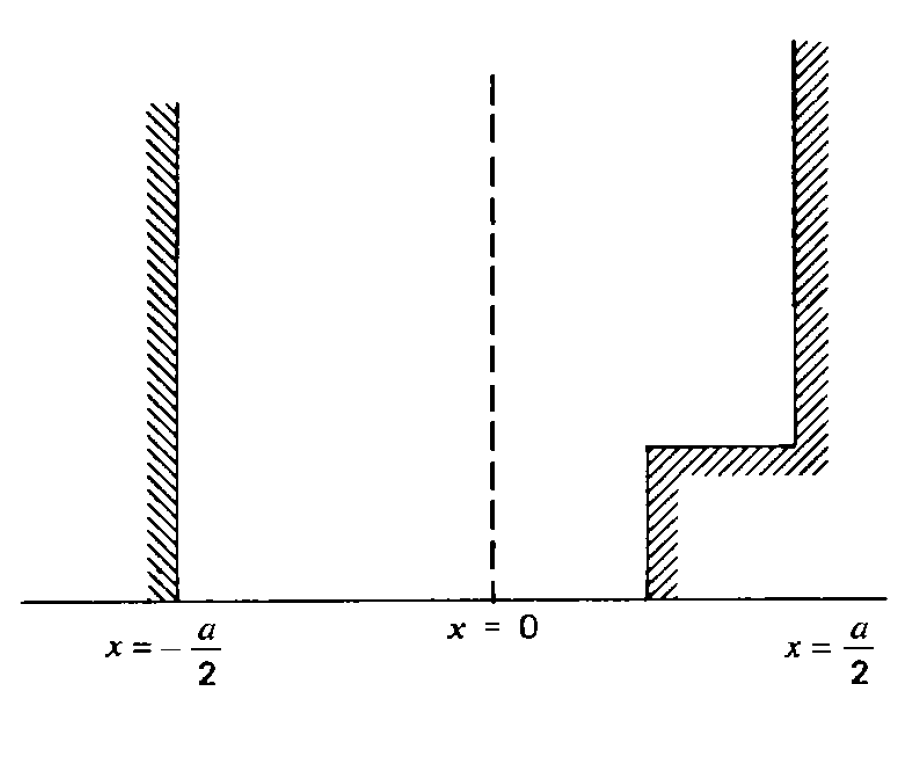
\includegraphics[width=0.5\linewidth]{figurler/non_symmetric_pot.png}
	\caption{\YAZILACAK, değişecek veya silinecek...}
	\label{fig:nonSymmetricPot}
\end{figure}

Şekil \ref{fig:nonSymmetricPot}'deki gib bir sistemin bir çift özfonksiyonu başlangıçta ($t=0$'da),
%%
\begin{equation}
\psi(x, 0)=\psi(-x, 0) \equiv \psi^{(+)}(x)
\end{equation}
%%
olarak tanımlanabilir. Bu sistemin zamanla gelişimi,
%%
\begin{equation}
i \hbar \frac{\partial \psi(x, t)}{\partial t}= \hat H \psi(x, t)
\end{equation}
%%
ile tanımlanır. Bu denkleme $\hat P$ işlemcisi uygulanırsa,
%%
\begin{equation}
i \hbar \frac{\partial}{\partial t} \hat P \psi(x, t)= \hat P  \hat H \psi(x, t)
\end{equation}
%%
elde edilir. Eğer $\hat H$, $x \rightarrow -x$ yansıması altında, çift kalıyorsa (V(x) ve $\frac{d^2}{dx^2}$ çift ise bu mümkündür);
%%
\begin{equation}
i \hbar \frac{\partial}{\partial t}[ \hat P \psi(x, t)]= \hat H[ \hat P \psi(x, t)]
\end{equation}
%%
sonucuna ulaşılır. Böylece
%%
\begin{equation}
\psi^{(+)}(x, t)=\frac{1}{2}(1+ \hat P) \psi(x, t) \quad \text{ ve } \quad \psi^{(-)}(x, t)=\frac{1}{2}(1- \hat P) \psi(x, t) 
\end{equation}
%%
Schrödinger denklemini birbirinden bağımsız olarak sağlayan bu iki çözüm önerilebilir. Çözümlerin zamanla bir birine karışmayacağı ve sistemin ilk durumu ne olursa olsun ilk durumun zamanla değişmeden korunacağı iki çözüm elde edilmiş olur.
Paritenin zamanla değişmezliğini bütün mümkün durumlar için aşağıdaki eşitlğin sağlanması garanti altına alır. 
%%
\begin{equation}
( \hat P  \hat H-  \hat H  \hat P) \psi(x, t)=0
\end{equation}
%%
Bu eşitlik kısaca,
%%
\begin{equation}
[ \hat P,  \hat H]=0
\end{equation}
%%
olarak yazılabilir ve $\hat P$ ve $\hat H$ işlemcilerinin komütasyon özelliğini sağlaması şartı olarak adlandırılır.

Bu önemli şart oldukça genel bir ifadeyle ``zamana bağlılığı açık olmayan ve $\hat H$ Hamiltonyen ile komüte eden herhangi bir işlemci ilgili hareketin sabitidir" olarak tanımlanır. Örneğin potansiyel $V(x,t)$ şeklinde zamana bağlı ise enerji artık bir hareket sabiti olmaktan çıkar. Dahası, bu durmda Schrödinger denklemi zamana bağlı ve zamandan bağımsız kısım olarak ikiye ayrılamayacağından bir enerji özdeğeri denklemi de elde edilemez.

Özet olarak, dejenere özfonksiyonların birbirinden farklı olduklarınının gözlenmesini sağlayan aynı özfonksiyonların başka bir hermityen işlemcinin de özfonksiyonları olmalarıdır. Yukarıda bahsi geçen  $\hat p$ ve $\hat P$ işlemcilerinin her ikisi de $\hat H$ Hamiltonyen işlemcisiyle komüt edebilirler. Her iki işlemci de $\hat H$ ile komütasyon şartını sağladıklarından $\hat H$'nin özfonsiyonları bu iki işlemcinin de eşzamanlı özfonksiyonlarıdır. Fakat bu durumun aksine $\hat p$ ve $\hat P$ komüt etmezler bu nedenle özfonksiyonları aynı değildir.



%%\newpage
% In the preamble, add "\renewcommand\refname{New Title}" for article type documents 
% and "\renewcommand\bibname{New Title}" for book and report type documents.
\renewcommand\refname{Kaynaklar}
\bibliography{quantumBIB}{}
%% https://www.sharelatex.com/learn/latex/bibtex_bibliography_styles
 \bibliographystyle{plain}
%% \bibliographystyle{alpha}
%%\bibliographystyle{apalike}
\end{document}

